\chapter{The Central Limit Theorem in Action}

\setcounter{problem}{1}

\section{Discussion}

\begin{fullwidth}

The goal of this lab is to observe how the sample means of uniform and exponential random variables have normal distributions with $N(\mu, \sigma^2/n)$ where $\sigma^2$ is the variance of the underlying distribution. Use filenames {\tt clt\_unif.py}, {\tt clt\_exp.py} for this lab.

\section{CLT applied to uniform random variables}

\subsection{Steps}

\step Import the usual libraries and then define these constants:

\begin{pyverbatim}
N = 4  # sample size
TRIALS = 500 # how many samples we will take from the uniform distribution
\end{pyverbatim}

Now, we need to build a loop that fills an {\tt X\_} list of length {\tt TRIALS}.  We will compute {\tt TRIALS} means of {\tt X}, which is a sample of size $N$ from $U(0,1)$. \\

\step Init {\tt X\_} to an empty list

\step Make a loop that goes around {\tt TRIALS} times

\step Inside the loop, get a sample of $N$ random values from $U(0,1)$ into list $X$.

\step Compute the mean of $X$ and append to the {\tt X\_} list.

\step Plot the histogram of {\tt X\_}:

\begin{pyverbatim}
# plot density of means (normalized histogram of means)
# WARNING: bins=40 is to show changes in resolution
#          where normally it's best to let the hist()
#          choose the bins for smoother view
plt.hist(X_, bins=40, normed=1)
\end{pyverbatim}

\step Run it. It should look like this \\

\scalebox{.35}{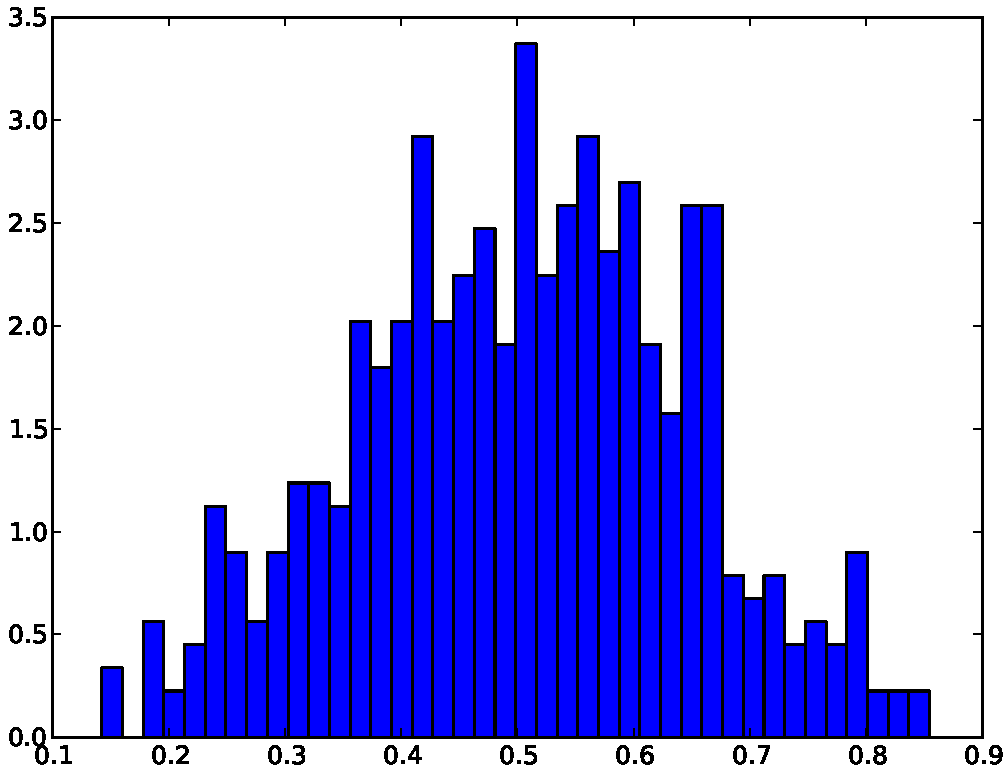
\includegraphics{figures/clt_unif-500-4-basic.pdf}}

Cool. it looks kind of like a normal distribution to me. Let's add the theoretical normal distribution on top. To do that we need the appropriate parameters. The mean of uniform samples should be midway between $a$ and $b$ from $U(a,b)$. In our case, that's 0.5. The variance of the uniform distribution is $(b-a)^2/12$ and we need the variance divided by sample size $N$. \\

\step  Let's get started on the theoretical distribution by defining a function called {\tt varunif(a,b)} that returns the variance of the uniform distribution from {\tt a}..{\tt b}.  

\step Then, plot the theoretical normal distribution and set the axes so that we can use the same range throughout the next series of tests to see how the distribution changes. Note that the normal distribution from scipy expects the standard deviation not the variance and so we need the square root.

\begin{pyverbatim}
# plot real normal curve N(0.5, sigma^2/n)
x = np.arange(0, 1.1, 0.01)
y = stats.norm.pdf(x, 0.5, FILL THIS IN))
plt.axis([.1,.9,0,7])
plt.plot(x,y, color='red')
\end{pyverbatim}

\step Run it. The resulting graph should look like this \\

\scalebox{.35}{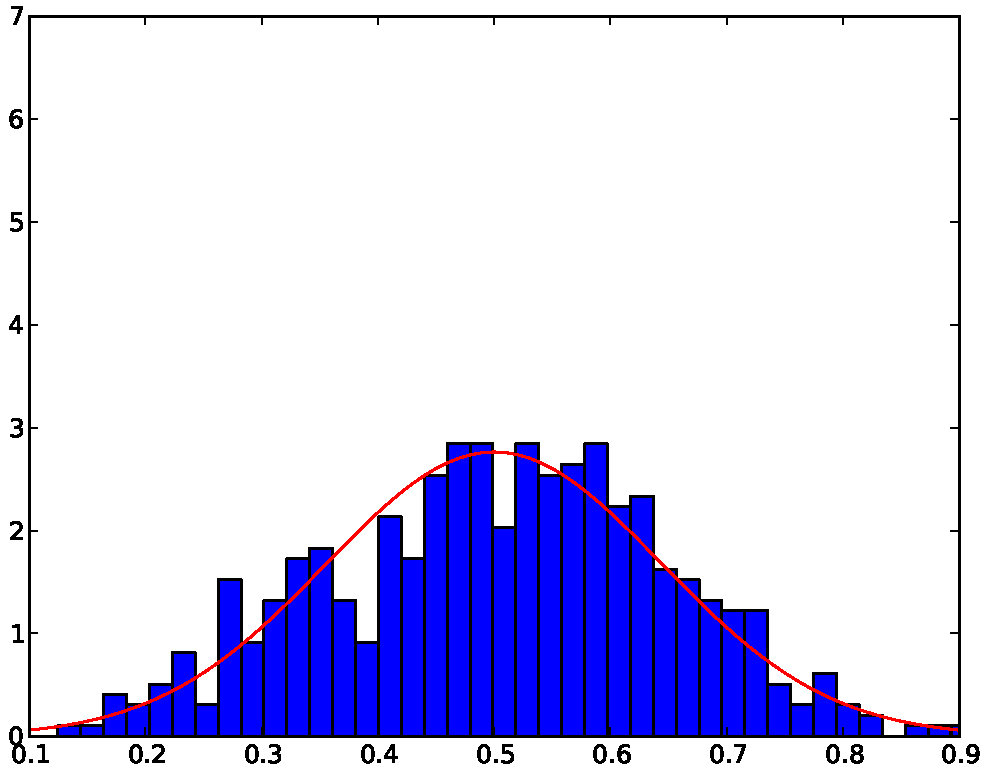
\includegraphics{figures/clt_unif-500-4-fancy.pdf}}

\step Now, display some important parameters in the graph using {\tt text()}. You will need to do that {\tt fig.add\_subplot(111)} thing again early in your script. The text in between the \$ symbols is latex and lets us display nice math symbols (e.g., the title), although I'm not doing much with it here.

{\small
\begin{pyverbatim}
plt.text(.02,.9, '$N = %d$' % N, transform = ax.transAxes)
plt.text(.02,.85,'$TRIALS = %d$' % TRIALS, transform = ax.transAxes)
plt.text(.02,.8, 'mean($\\overline{X}$) = %f' % np.mean(X_), transform = ax.transAxes)
plt.text(.02,.75,'var($\\overline{X}$) = %f' % np.var(X_), transform = ax.transAxes)
plt.text(.02,.7, 'var U($0,1$)/%d = %f' % (N,varunif(0,1)/N), transform = ax.transAxes)

plt.title("CLT Density Demo. sample mean of U(0,1) is $N(.5, \sigma^2/N)$")
plt.xlabel("$\\overline{X}$", fontsize=16)
plt.ylabel("Density", fontsize=16)
\end{pyverbatim}
}

\step Run it. The resulting graph should look like this \\

\scalebox{.35}{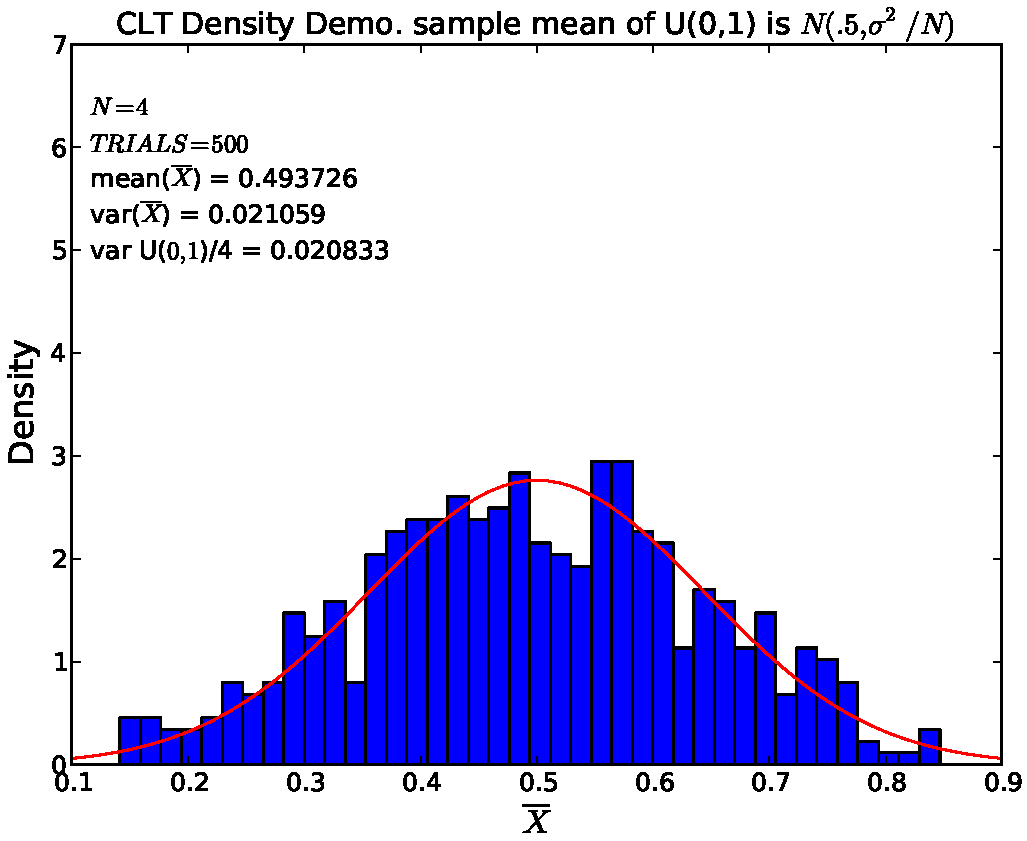
\includegraphics{figures/clt_unif-500-4-fancier.pdf}}

Notice how the mean is close to the expected 0.5 and that the variance of the sample mean is close to the theoretical variance.\\

\step Increasing the number of trials two 2000 shows much higher resolution but does not change the variance/tightness of the distribution at all. Run it and see the following:

\scalebox{.35}{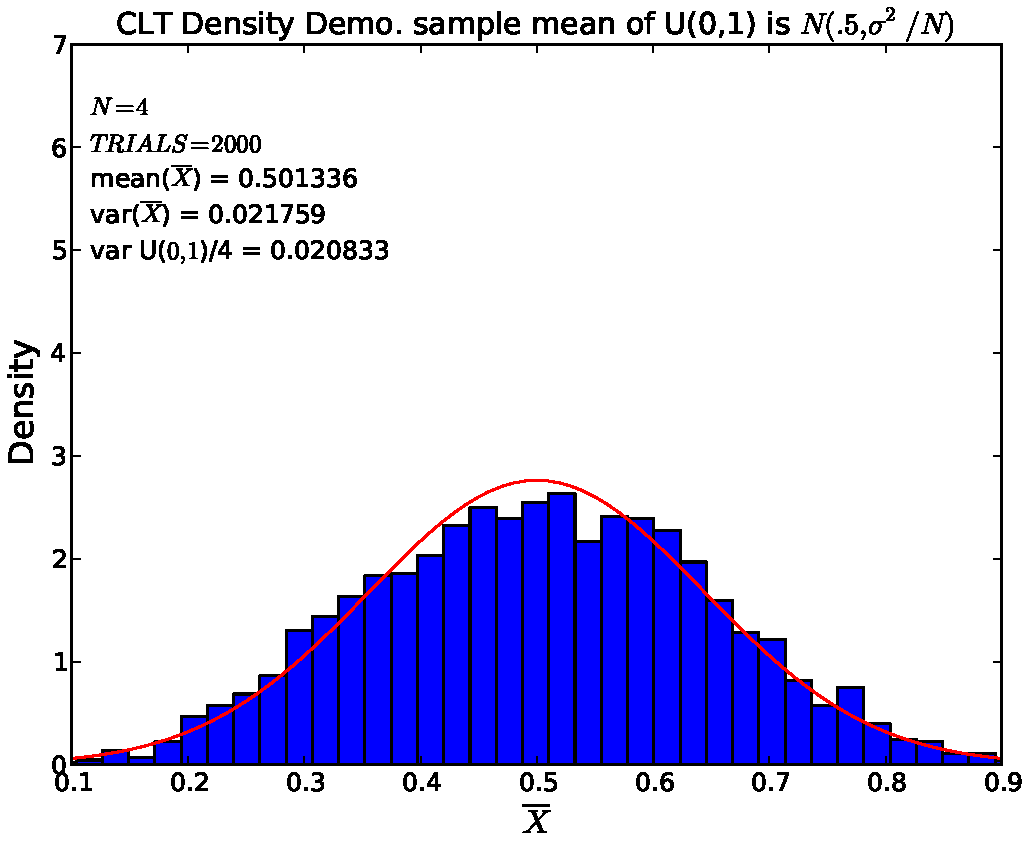
\includegraphics{figures/clt_unif-2000-4.pdf}}

\step Now, if we increase the sample size to $N=10$, we get a much tighter variance on the mean of $\overline{X}$. Run it:

\scalebox{.35}{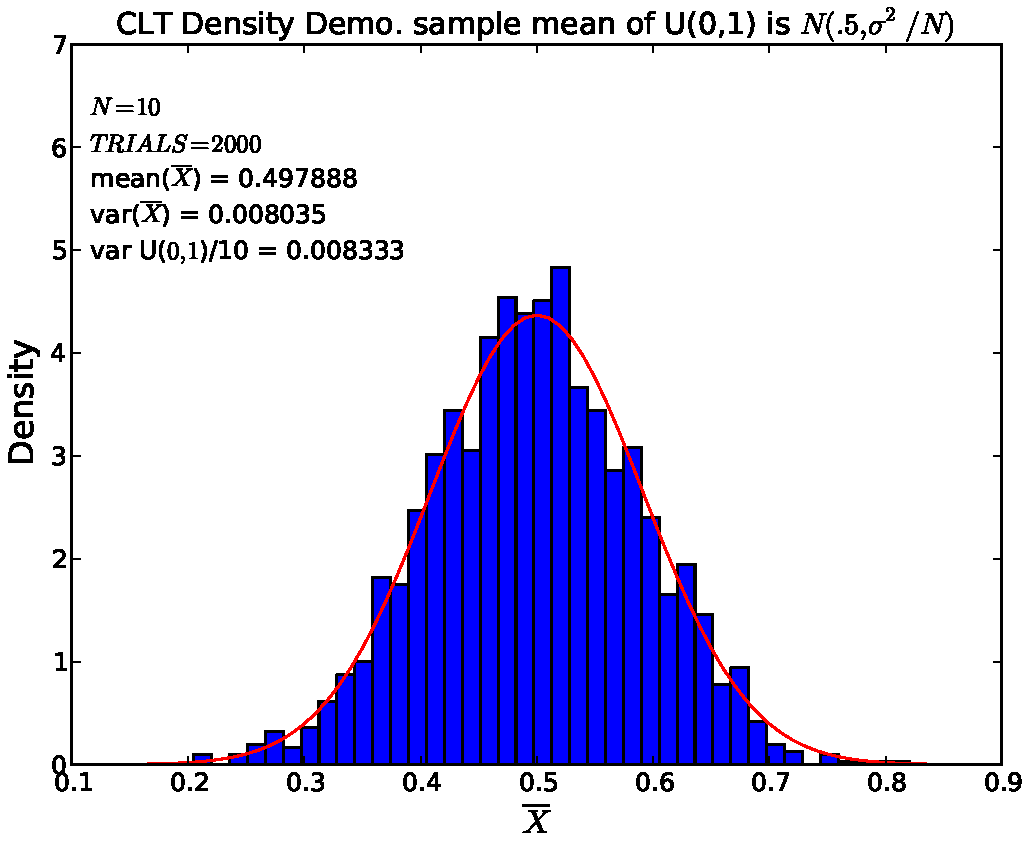
\includegraphics{figures/clt_unif-2000-10.pdf}}

\step Increasing to 20 we get:

\scalebox{.35}{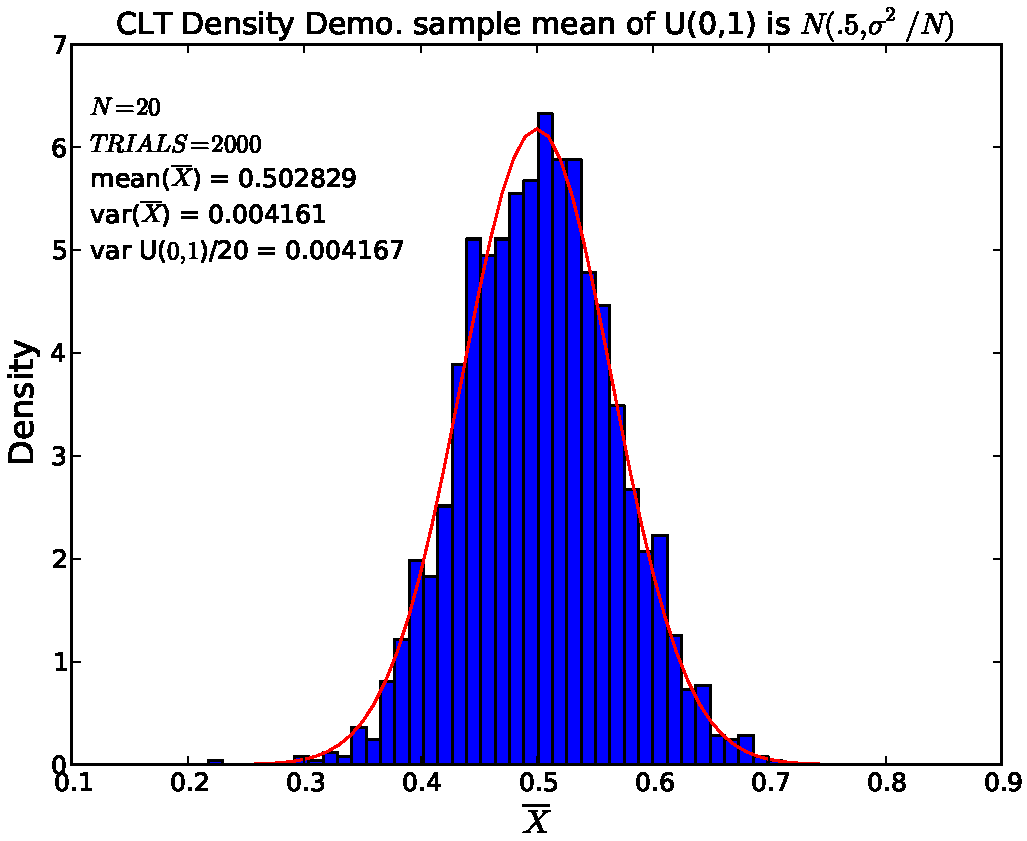
\includegraphics{figures/clt_unif-2000-20.pdf}}

\section{CLT applied to exponential random variables}

Now let's look at how the central limit theorem still gives us a normal distribution even when we pull random variables from a skewed distribution like the exponential.

\subsection{Steps}

\step Grab the {\tt rexp(lambduh)} function you wrote for a previous lab to get exponential random variables and start out with the following constants:

\begin{pyverbatim}
N = 10
TRIALS = 4000
LAMBDUH = 1.5
\end{pyverbatim}

\step Repeat the loop we did above to get the mean of a bunch of samples. This time, use {\tt rexp(LAMBDUH)} instead of the uniform distribution function.

\step Here is how to plot the theoretical normal distribution on top:

\begin{pyverbatim}
# plot real normal curve N(1/lambda, sigma^2 / N)
x = np.arange(0, 1.1, 0.01)
y = stats.norm.pdf(x, FILL IN MEAN, FILL IN STDDEV)
plt.plot(x,y, color='red')
\end{pyverbatim}

\step Here are the appropriate text annotations:

{\small
\begin{pyverbatim}
plt.text(.02,.9, '$N = %d$' % N, transform = ax.transAxes)
plt.text(.02,.85, '$TRIALS = %d$' % TRIALS, transform = ax.transAxes)
plt.text(.02,.8,   'mean($\\overline{X}$) = %f' % np.mean(X_), transform = ax.transAxes)
plt.text(.02,.75, 'var($\\overline{X}$) = %f' % np.var(X_), transform = ax.transAxes)
plt.text(.02,.7, 'mean Exp($%f$) = %f' % (LAMBDUH,1/LAMBDUH), transform = ax.transAxes)
plt.text(.02,.65, 'var Exp($%f$)/%d = %f' % (LAMBDUH,N,(1/LAMBDUH**2)/N), transform = ax.transAxes)

plt.title("CLT Density Demo. sample mean of Exp($\lambda=1.5$) is $N(1/\lambda, (1/\lambda^2)/N)$")
plt.xlabel("$\\overline{X}$", fontsize=16)
plt.ylabel("Density", fontsize=16)
plt.axis([0,1.333,0,5])
plt.savefig('clt_exp-'+str(TRIALS)+'-'+str(N)+'.pdf', format="pdf")
\end{pyverbatim}
}

\step Run it and you should see the following two graphs according to the value of $N$:

\noindent \scalebox{.33}{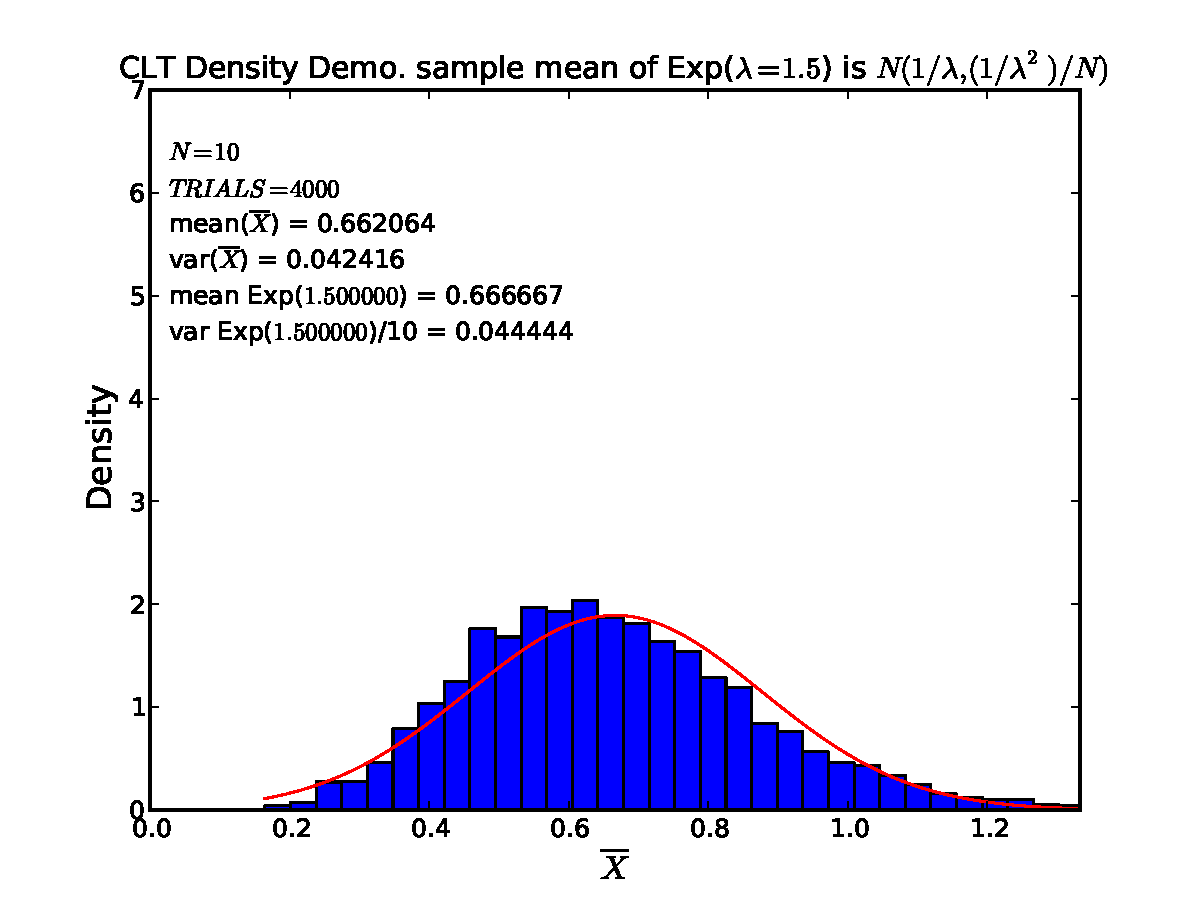
\includegraphics{figures/clt_exp-4000-10.pdf}} \scalebox{.33}{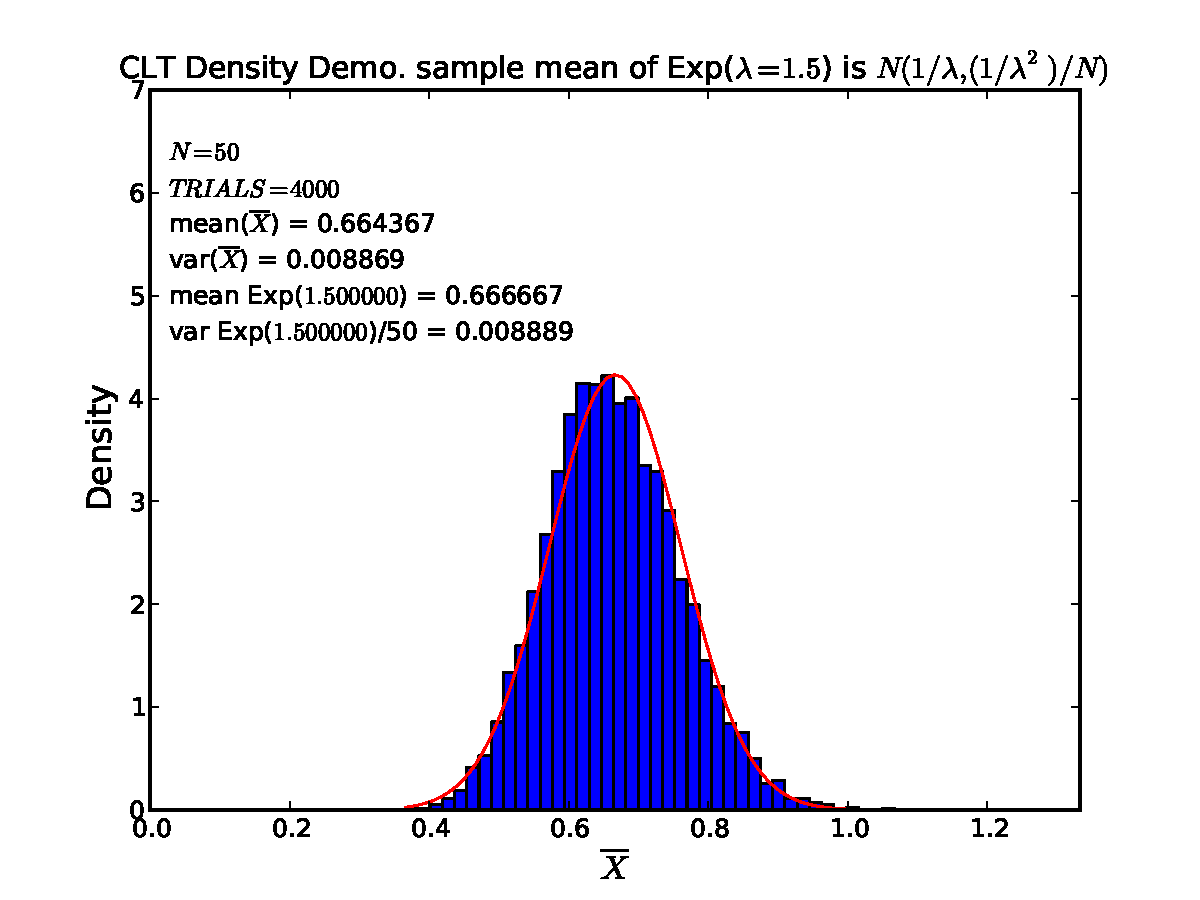
\includegraphics{figures/clt_exp-4000-50.pdf}}

Notice that there is a slight leftward bias in that the normal distribution is a little bit to the right it looks like. This is to be expected. You really need to bump up $N$ before you see it converge to the proper alignment.\\

\step Play around with other values of lambda and N.

\section{Deliverables}

Please submit:

\begin{itemize}
\item both Python files
\item a PDF for $N=20$, $TRIALS=2000$ for CLT $U(0,1)$ demo
\item a PDF for $N=50$, $TRIALS=4000$, $\lambda=1.5$ for CLT $Exp(\lambda)$ demo
\end{itemize}

\end{fullwidth}
